\documentclass[12pt]{article}
\usepackage{times}
\usepackage[most]{tcolorbox}
%Bibliography   
    \usepackage{apacite}
    \bibliographystyle{apacite}
    %http://www.ctan.org/tex-archive/biblio/bibtex/contrib/apacite/apacite.pdf
 
%Essay Header
	\pagestyle{myheadings}
	\markright{\hfill \emph{Horowitz }}

%pdfLaTeX: TeX Gyre Termes
	%\usepackage{tgtermes}
	\usepackage[T1]{fontenc}

%Sectioning
    \usepackage{sectsty}
    \sectionfont{\fontsize{13}{15}\selectfont}

%Packages
    \usepackage[margin=1in]{geometry}
    \usepackage{setspace}
    \usepackage[leftmargin = 1in, rightmargin = 0in, vskip = 0in]{quoting}
    \usepackage{microtype}



\doublespacing

\begin{document}
\begin{center}
Modeling Apartment Sale Prices in Queens\\~\\
\footnotesize Final project for Math 390 Data Science at Queens College\\
May 24, 2020
\end{center}

\begin{flushright}
By Tziporah Horowitz\\
\end{flushright}

\subsubsection*{Abstract}

The goal of this paper is to create a predictive model for the sale price of apartments in Queens, New York. Using data on the Queens housing market between February 2016 and February 2017, three predictive models were made via the OLS, Regression Tree, and Random Forest algorithms. By identifying key explanatory features, the three models are obtained and discussed in detail. Of the three, only the Random Forest model is accurate enough to be used in the real world.

\pagebreak



\subsection*{1. Introduction}

%Write about the problem here and some context and background. No need to cite papers. Talk about what a predictive model is and what that means here. What is the unit of observation? What is the response? Write about the basics of how you modeled it. You can mention your performance results, but do not go into detail about them (leave it for the discussion section). Use as much vocabulary as you can from the class notes and your previous writing assignment in describing the problem. Cite sources in APA style, i.e Johnson et al. (1999) within text and (Johnson et al., 1999) within a parenthetical.

As one of the four outer-boroughs of New York City and the most ethnically diverse urban area in the world, Queens County sees a large variation in real estate sale prices each year. Zillow.com tries to make estimates of housing sale prices in a given location, but they are often inaccurate and do not apply to Queens. Using data obtained from the Multiple Listing Service of Long Island, this paper aims to predict the sale price of Queens apartments by modeling sales below \$1,000,000 between February 2016 and February 2017.

Mathematical models are abstractions of reality expressed as functions of measurable data, used to explain or predict future events of phenomena. Although models inherently contain error due to the nature of unknown causation, they can be useful when metrics of a phenomenon's causal features are defined to minimize the error. Even with, properly defined features, the model will not be meaningful without a hypothesis set ($\mathcal{H}$) to allow for various algorithms that can form predictions. Using the \emph{Regression Tree}, \emph{OLS}, and \emph{Random Forest} algorithms, this paper defines three models for predicting the sale price of apartments in Queens.




\subsection*{2. The Data}

The data obtained from www.MLSLI.com via Amazon's MTurk has 2,330 rows and 55 columns of character, logical, and numerical type. After importing the data to RStudio running R 3.6.3, the columns created by MTurk regarding the download process were immediately dropped, leaving 31 character and numerical features. Of the 2,330 rows, only 528 contain values and can be used for prediction. Before dropping the unusable $NA$ values of sale price, other columns were cleaned and imputed when necessary. After the data wrangling process, additional data from public.opendatasoft.com was merged via left join on the original dataset to provide three more columns of meaningful location data for each zip code.




\subsubsection*{2.2. Featurization}

%How many and what measurements did you take on the observations? Which were provided to you in the raw data and which did you featurize yourself? Make sure to list them and give a brief explanation as to what they are; describe what these measurements capture about the observation. Give a basic summary of each feature --- average, standard deviation, range for those that are continuous data type and percentages of the categories for those that are nominal data type.

From the 34 columns in the new dataset, \codeword{sale_price} was removed and set aside as \codeword{y}, the response variable. Of the remaining columns, 17 were selected for featurization; 6 binary or categorical and 11 numeric. 

The categorical variables include \codeword{dining_room_type}, \codeword{fuel_type}, \codeword{kitchen_type}, \codeword{cats_allowed}, \codeword{condo_coop}, and \codeword{season}; \codeword{dogs_allowed} was not included in the linear model because it presented collinearities with another variable. \codeword{dining_room_type} is a factor of four categories: combo, formal, dining area, and other. \codeword{fuel_type} is also a factor of four categories: oil, gas, electric, and other. \codeword{cats_allowed} is a binary variable: 1 if cats are allowed in the building and 0 otherwise. \codeword{coop_condo} is also a binary variable: 1 if the apartment is a co-op and 0 if it is a condo. All of the categorical variables except for \codeword{season} were from the original dataset. \codeword{season} was creating by extracting the month of sale from \codeword{date_of_sale} and placing them in four bins: winter, spring, summer, and fall.

The numeric variables include \codeword{parking_charges}, \codeword{sq_footage}, \\ \codeword{num_floors_in_building}, \codeword{approx_year_built}, \codeword{community_district_num}, \\ \codeword{num_bedrooms}, \codeword{num_full_bathrooms}, 
\codeword{num_total_rooms}, \codeword{total_maintenance},
\codeword{Latitude}, and \codeword{Longitude}. 
\codeword{parking_charges} is the total amount of parking fees associated with a given apartment, expressed on dollars. \codeword{num_floors_in_building} is the number of floors in the building, ranging from 1 to 34. \codeword{sq_footage} is the area of the apartment in ft$^2$. \codeword{approx_year_built} is the year that the building was in, ranging from 1915 to 2016. \codeword{community_district_num} is the community district number that the apartment is located in. \codeword{num_bedrooms} is the number of bedrooms in the apartment, ranging from 0 to 3. \codeword{num_full_bathrooms} is the number of full bathrooms in the apartment, ranging from 1 to 3. \codeword{num_total_rooms} is the number of total rooms in the apartment, ranging from 1 to 8. All variables except for \codeword{total_maintenance},
\codeword{Latitude}, and \codeword{Longitude} were from the original dataset. \codeword{total_maintenance} is a combined metric of maintenance fees, common charges, and total taxes, differing between co-ops and condos. \codeword{Latitude} and \codeword{Longitude} are the geographic coordinates from the additional location dataset, based on the postal code provided in the url of each observation.


\subsubsection*{2.3. Errors and Missingness}

%Did you find obvious errors (not missingness) in the dataset? How did you handle these errors? Summarize the missingness across the features in Section 2.2. How did you handle missingness in your data? Talk about how you imputed. Did you include any missingness dummy variables in your expanded feature set? Note: you do not need to explain how you handled missingness in your prediction set.

Prior to feature selection, there were many spelling errors in categorical variables. For example, the \codeword{cats_allowed} column originally contained three levels: "yes," "y," and "no." The column was then converted to a binary, 1 if \codeword{cats_allowed} was "yes" or "y" and 0 if it was "no." Other columns like \codeword{parking_charges} were imported as strings like "\$1,000" where the "\$" and "," needed to be removed to convert the variable to numeric type. Lastly, columns like \codeword{date_of_sale} had to be converted from character type to date-time so that it could be used numerically.

Once the non-missing values of the variables were made meaningful, the $NA$ values could be dropped or imputed. $NA$ values in each column were only omitted if there were fewer than 20 missing observations for the feature. After those observations were removed, a subset of the dataset was created by selecting the rows in which \codeword{y} was not missing. In this subset, there were 513 remaining rows of data and 6 columns that still contained missing values. The \codeword{pct_tax_deductibl} column was removed from the dataset completely because there were too many $NA$ values. Missingness dummies for the 5 columns with missing values were added to the feature set after imputation to see if there is meaning in the missing data. The missing values were imputed in the full dataset using the \codeword{missForest} library, starting with the column with the fewest $NA$'s.

\subsection*{3. Modeling}

%You are creating a model to ship to the world to be used for predicting real, new observations. But you also would like to explore a little bit.

Using a subset of the imputed dataset concatenated with the missingness dummies where \codeword{y} is not missing, three models were built to comparatively predict the sale price of Queens apartments.

\subsection*{3.1 Regression Tree Modeling}

%Fit one regression tree. Visualize the top layers. Comment on the top 10 features that are seemingly most important for predicting sale price. Include the visualization as a figure.  If you cannot get \texttt{YARF} to work, use the canonical CRAN package \texttt{rpart}.

Regression trees are used to create step-wise models for prediction using split rules. The algorithm iteratively considers every possible orthogonal-to-axis split and selects the split rule with the smallest Weighted Sum of Squared Error $\big( SSE_{weighted} = \frac{n_l SSE_l + n_r SSE_r}{n_l + n_r}$ where $l$ is the left of the split and $r$ is the right$\big)$ for node construction. Using the \emph{Regression Tree} algorithm, a model was constructed with 21 layers, 157 leaves, and 313 nodes. 

\begin{figure} 
\centering
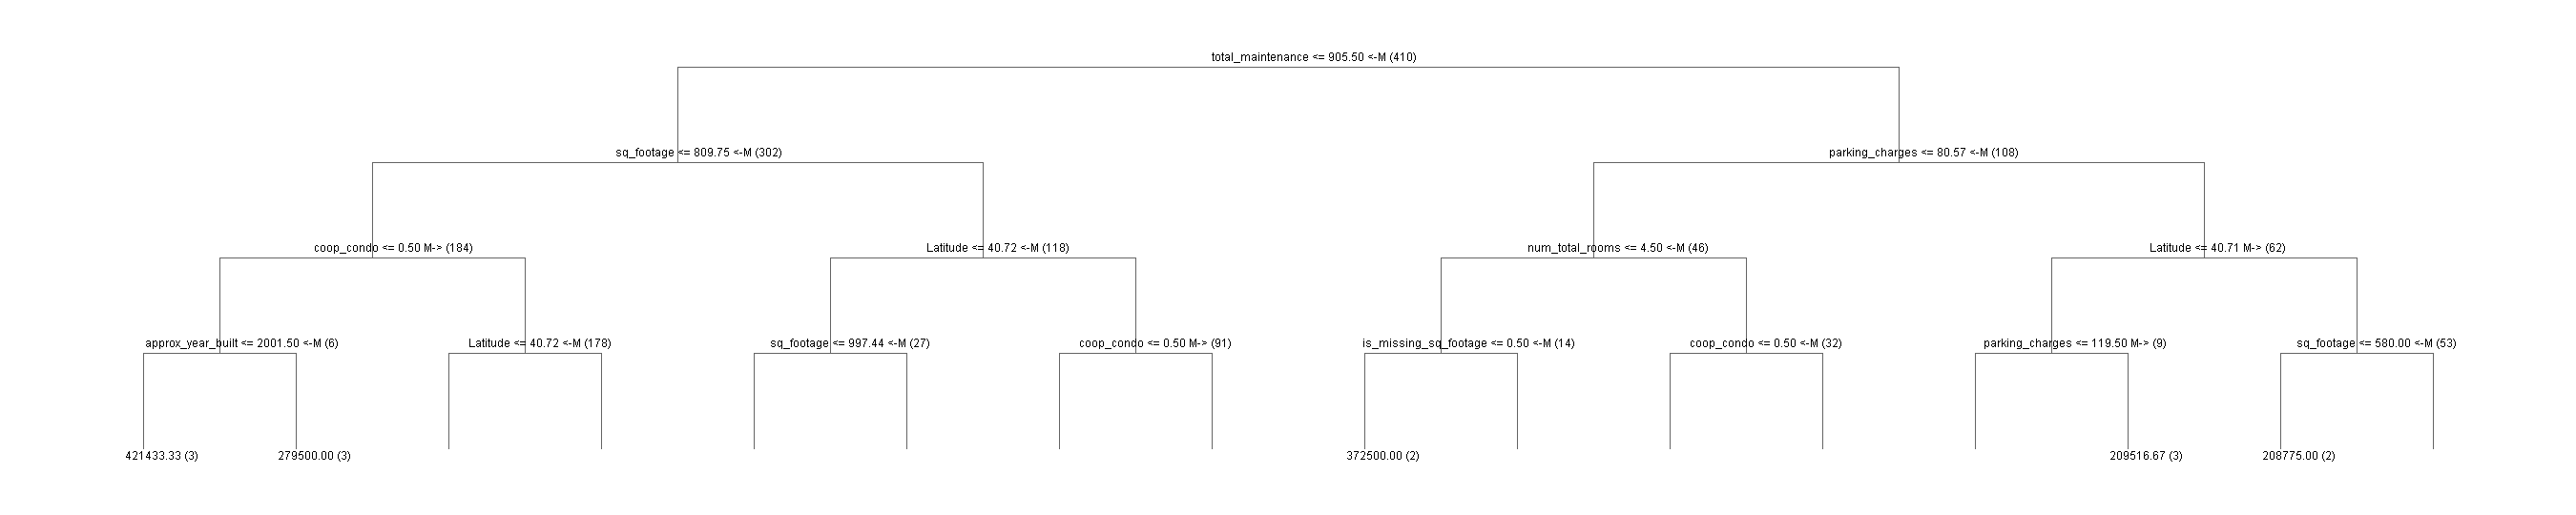
\includegraphics[scale = .5]{yarf_mod_tree_1.png} 
\caption{First three layers of the regression tree model}
\label{regression tree}
\end{figure} 

Figure \ref{regression tree}. shows the first three layers of the tree. Starting from the root node, the most important split rule is \codeword{total_maintenance} less than or equal to \$905.50. This is likely because apartments with higher maintenance fees often sell at lower prices. In an apartment with lower maintenance fees, the next most significant feature is \codeword{sq_footage}  less than or equal to 801.59 ft$^2$. In general, apartments with smaller square footage cost less than apartments with significantly more; however, because there are many other factors determining sale price, it is not a rule of thumb. If the square footage is below the split, the next split is on \codeword{coop_condo}, likely due to both the difference in price and maintenance fees between them. Co-ops tend to be cheaper per square foot but have both property tax and maintenance costs while condos only have common charges. Following the apartment type, the tree splits into two nodes: \codeword{Longitude} less than or equal to $-73.82^{\circ}$ for condos and \codeword{Latitude} less than or equal to $40.72^{\circ}$ for co-ops. The apartment's geographical location plays an important role in predicting sale price as apartments closer to Manhattan often cost more than those farther away. Furthermore, apartments in low-income geographical areas cost less than those in high-income neighborhoods. \codeword{Latitude} less than or equal to $40.72^{\circ}$ is also used as a split rule when \codeword{sq_footage} is greater than 801.59 ft$^2$. Following this split, the tree breaks off into \codeword{sq_footage} less than or equal to 940.56 ft$^2$ on the left and \codeword{approx_year_built} before 1986 on the right.

On the right side of the tree in Figure \ref{regression tree}., the first split rule after \codeword{total_maintenance} greater than \$905.50 is \codeword{parking_charges} less than or equal to \$75.44. This is likely because higher parking fees tend to raise the sale prices of apartments. If parking fees are low, the next split is \codeword{num_bedrooms} less than 2, as sale price tends to increase with the number of bedrooms in an apartment. Following \codeword{num_bedrooms}, the tree splits into \codeword{approx_year_built} before 1957 on the left and \codeword{Longitude} less than or equal to $-73.84^{\circ}$. Geographical location also plays a large role on the right of \codeword{parking_charges}, with \codeword{Latitude} less than or equal to $40.70^{\circ}$ leading to the tree's first leaf, a predicted sale price of \$183,900. However, if \codeword{Latitude} is greater than $40.70^{\circ}$, the tree continues to split on \codeword{sq_footage} less than or equal to 580 ft$^2$. Although there are too many nodes for the human eye to interpret, observing the regression tree can help one understand which features are most important.



\subsection*{3.2 Linear Modeling}

%Fit a vanilla OLS linear model. Comment on its in-sample error statistics and interpret them. For the most important features found in the regression tree, interpret the coefficients in this model. Will a linear model be good for prediction? Include the OLS output as a table.

Linear models are useful because they provide meaningful interpretations and error metrics. Table \ref{linear_mod}. shows the regression outputs of the model, \codeword{y ~ 0 + X_train}. The linear model has an in-sample $R^2$ of 95.78\% and an RMSE of $\pm$\$55,500. The in-sample error metrics suggest that the model predicts well; however, when comparing the standard error of the residuals in-sample (\$53,721.85) and out-of-sample (\$126,121.10), the model largely overfits, indicating that it will not perform well in the future. 

According to the in-sample model, sale price decreases by \$0.76 for each dollar of maintenance fees when all other variables are held constant. This enforces the theory stated earlier that apartments with higher maintenance fees sell at lower prices\footnote{It is important to note however, that while the regression tree suggests total\_maintenance is an important feature, the linear model suggests it is insignificant based on a p-value of 0.86.}. The model similarly asserts the assumption that the larger the square footage of the apartment, the higher the sale price tends to be. When all other variables are held constant, sale price increases by \$136.09 for each square foot. The linear model also suggests that apartment type plays a large role in predicting sale price; if the apartment is a co-op, sale price decreases by \$168,053.00 when all other variables are held constant. The geographic estimates indicate that sale price increases by \$889,756.81 per degree of latitude and decreases \$108,243.26 per degree of longitude\footnote{Because geographical coordinates vary by hundredths of degrees in Queens, these coefficients do not change sale prices as drastically as they suggest.}. Like the regression tree model, this model suggests that sale prices increase significantly by \$361.87 for each dollar of parking fees.


% latex table generated in R 3.6.3 by xtable 1.8-4 package
% Sun May 24 19:38:41 2020
\begin{table}[ht]
\centering
\caption{Linear Model (In-Sample)} \label{linear_mod}
\begin{tabular}{rrrrr}
  \hline
 & Estimate & Std. Error & t value & Pr($>$$|$t$|$) \\ 
  \hline
parking\_charges & 361.8722 & 82.7363 & 4.37 & 0.0000 \\ 
  sq\_footage & 136.0939 & 32.8910 & 4.14 & 0.0000 \\ 
  dining\_room\_typecombo & -42811915.3953 & 7652419.2110 & -5.59 & 0.0000 \\ 
  dining\_room\_typedining area & -42843715.9091 & 7656467.5956 & -5.60 & 0.0000 \\ 
  dining\_room\_typeformal & -42806314.6291 & 7652835.4925 & -5.59 & 0.0000 \\ 
  dining\_room\_typeother & -42792148.1625 & 7653466.9771 & -5.59 & 0.0000 \\ 
  num\_floors\_in\_building & 4446.3163 & 680.0970 & 6.54 & 0.0000 \\ 
  fuel\_typegas & -8331.6065 & 23975.7382 & -0.35 & 0.7284 \\ 
  fuel\_typeoil & -5804.8785 & 24317.7857 & -0.24 & 0.8115 \\ 
  fuel\_typeother & 6005.0612 & 31748.3807 & 0.19 & 0.8501 \\ 
  approx\_year\_built & -686.4603 & 283.9789 & -2.42 & 0.0161 \\ 
  cats\_allowed & 18789.1958 & 5902.9989 & 3.18 & 0.0016 \\ 
  community\_district\_num & 1888.4452 & 1005.4334 & 1.88 & 0.0611 \\ 
  coop\_condo & -168053.0069 & 15393.7237 & -10.92 & 0.0000 \\ 
  kitchen\_typeeat in & -1033.1223 & 9249.0530 & -0.11 & 0.9111 \\ 
  kitchen\_typeefficiency & -13387.4088 & 8975.0735 & -1.49 & 0.1366 \\ 
  num\_bedrooms & 35740.8667 & 7396.8283 & 4.83 & 0.0000 \\ 
  num\_full\_bathrooms & 20349.4848 & 14492.5098 & 1.40 & 0.1611 \\ 
  num\_total\_rooms & 6802.4141 & 5109.9016 & 1.33 & 0.1839 \\ 
  seasonspring & -12399.4676 & 8266.8543 & -1.50 & 0.1345 \\ 
  seasonsummer & -14199.6609 & 8168.4213 & -1.74 & 0.0830 \\ 
  seasonwinter & 4328.8330 & 8083.6936 & 0.54 & 0.5926 \\ 
  Latitude & 889756.8071 & 97643.0803 & 9.11 & 0.0000 \\ 
  Longitude & -108243.2589 & 71552.8031 & -1.51 & 0.1312 \\ 
  total\_maintenance & -0.7567 & 4.3879 & -0.17 & 0.8632 \\ 
  is\_missing\_dining\_room\_type & -133.4281 & 7021.3286 & -0.02 & 0.9848 \\ 
  is\_missing\_fuel\_type & -6043.4737 & 14653.0562 & -0.41 & 0.6803 \\ 
  is\_missing\_num\_floors\_in\_building & -879.8882 & 7240.2965 & -0.12 & 0.9033 \\ 
  is\_missing\_parking\_charges & -3605.1479 & 6821.8142 & -0.53 & 0.5975 \\ 
  is\_missing\_sq\_footage & -7630.8312 & 6276.4969 & -1.22 & 0.2248 \\ 
   \hline
\end{tabular}
Residual standard error: 55500 on 380 degrees of freedom \\
Multiple R-squared:  0.9578,	Adjusted R-squared:  0.9545 \\
F-statistic: 287.5 on 30 and 380 DF,  p-value: < 2.2e-16 
\end{table}


\subsection*{3.3 Random Forest Modeling}

%Why should this be your choice of prediction model? Explain the theory as best as you could. Is it parametric / non-parametric? What did you gain by choosing this model? Lose? Was modeling an iterative process in some way? Do you think you underfit? Do you think you overfit? How were you able to know? Which variables do you believe have an effect on sale price that is truly causal, why and would you be able to prove it? Use the package \texttt{mlr} (or \texttt{mlr3}) to find the best tuning parameters for the RF model. Use these parameters to build the production model. If you cannot get \texttt{YARF} to work, use the canonical CRAN package \texttt{randomForest}.

\emph{Random Forest} is a non-parametric algorithm that utilizes \emph{Bootstrap Aggregating} or bagging to accurately make predictions out-of-sample. Bagging iteratively takes $m$ random samples of approximately $\frac{2}{3}$ of the original dataset with replacement and creates a new model with each sample. The algorithm then calculates the average of the models and its Mean Squared Error ($MSE = \sigma^2 + \rho \mathbb{E}_x \big[\text{Var}[g_{(m)}] \big]$ where $\rho$ is the average correlation between two trees, each built with a different bootstrap sample). \emph{Random Forest} aims to de-correlate the trees during node construction by splitting on a subset of features. By applying this algorithm to the Queens housing data, one can optimize prediction while shrinking the overfit based on the out-of-bag error metrics. 

\subsection*{4. Performance Results for your Random Forest Model}

The Random Forest model has an out-of-bag $R^2$ of 84.64\% and an out-of-bag RMSE of 70263.86; meaning the 95\% of the time the out-of-bag predictions are within $\pm$\$70,263.86 of  the true sale price. When creating a train-test split to estimate the generalization error of the model, out-of-bag $R^2$ was 83.34\% in-sample and 85.9\% out-of-sample. Furthermore, out-of-bag RMSE was 74749.7 in-sample and 61119.73 out-of-sample, indicating that the model slightly underfit but with low generalization error.

\begin{center}
Table 2: Error Metrics \\
\begin{tabular} {|c|c|c|} 
\hline
& $R^2$ & RMSE \\
\hline
$g_{train}$ & 83.34 & 74749.7 \\
$g_{test}$ & 85.9 & 61119.73 \\
$g_{final}$ & 84.64 & 70263.86 \\
\hline
\end{tabular}
\end{center}



%Report your oob goodness-of-fit metrics: $R^2$, $RMSE$ (no need for $MAE$ unless you want to report it) and interpret them. Report your estimate of generalization error as the same goodness-of-fit metrics: $R^2$, $RMSE$ and interpret these as well. How do you know this is a valid estimate of how the model will by-and-large perform on future predictions? In addition to using oob validation, do a hold-out test set validation as well and report the error metrics. Summarize these results in a figure or table.

\subsection*{5. Discussion}

%Discuss the project once again. Comment on things that you did informally (assume the reader has been through Sections 2-4). Talk about where you feel you fell short and how you can plug those holes. Talk about future extensions. Do you believe your model is production ready? Can you beat Zillow?

The goal of this paper was to create a model that can accurately predict apartment sale prices in the future. To do so, three models were created and discussed in detail. Although the Regression Tree model and Linear model are both inaccurate out-of-sample, they can be used to help a modeler understand the role of key explanatory variables. Although the Random Forest model could do better, it remains accurate out-of-sample and does better than Zillow's "zestimates."

While much of the limitations in the model may stem from misspecification error, the model was also largely limited by the dataset itself. The dataset started with 2,330 observations, but nearly 80\% of the rows had to be dropped due to the missing values of sale price. Further imputing was needed to model the remaining data points, but too much imputing can make the model dishonest. Although the dataset was usable, future enhancement to the training set, in terms of finding more data, removing unneeded variables, and finding new features can help create a better model with better predictive abilities.

\subsubsection*{References}

CivicSpace Labs. (2018, February 9). US Zip Code Latitude and Longitude. Open Data Soft. https://public.opendatasoft.com/explore/dataset/us-zip-code-latitude-and-longitude/table/?sort=-latitude.

\pagebreak

\subsubsection*{Code Appendix}

\includegraphics[scale = .8]{project-page-001.jpg} \pagebreak
\includegraphics[scale = .8]{project-page-002.jpg} \pagebreak
\includegraphics[scale = .8]{project-page-003.jpg} \pagebreak
\includegraphics[scale = .8]{project-page-004.jpg} \pagebreak
\includegraphics[scale = .8]{project-page-005.jpg} \pagebreak
\includegraphics[scale = .8]{project-page-006.jpg} \\



\end{document}
